% The Gaussian-integer lattice Z[i] (blue) together with one extra
% known lattice point 2.3 - 3.1i (red), for the third proof that O_K
% is a free Z-module.
% Source: book/tex/alg-NT/classgrp.tex (§ Third proof) — asy figure.
\documentclass[border=2mm]{standalone}
\usepackage{tikz}
\begin{document}
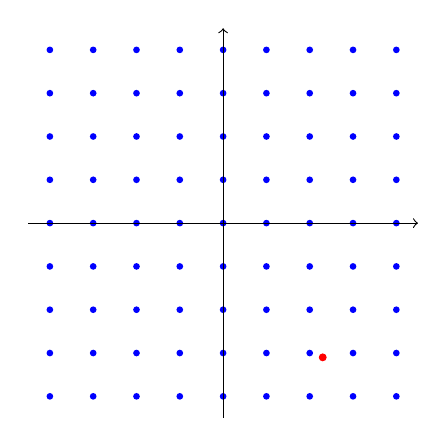
\begin{tikzpicture}[scale=0.55]
  \foreach \x in {-4,...,4}
    \foreach \y in {-4,...,4}
      \fill[blue] (\x,\y) circle (2.2pt);
  \fill[red] (2.3,-3.1) circle (2.6pt);
  \draw[->] (-4.5,0) -- (4.5,0);
  \draw[->] (0,-4.5) -- (0,4.5);
\end{tikzpicture}
\end{document}
